\documentclass[12pt]{article}
\usepackage{geometry}
\geometry{left=1in,right=0.75in,top=1in,bottom=1in}

%%%%%%%%%%%%%%%%%%%%%%%%%%%%%%%%%%%%%%%%
% Replace ABCDEF in the next line with your chosen problem
% and replace 1111111 with your Team Control Number
\newcommand{\Problem}{ABCDEF}
\newcommand{\Team}{1111111}
%%%%%%%%%%%%%%%%%%%%%%%%%%%%%%%%%%%%%%%%

\usepackage{newtxtext}
%\usepackage{hyperref}
\usepackage{amsmath,amssymb,amsthm}
\usepackage{lipsum}
\usepackage{booktabs}
\usepackage{float}

\usepackage[pdftex]{graphicx}
\usepackage{xcolor}
\usepackage{fancyhdr}
\usepackage{url}
\lhead{Team 2301831}
\rhead{}
\cfoot{}

\newtheorem{theorem}{Theorem}
\newtheorem{corollary}[theorem]{Corollary}
\newtheorem{lemma}[theorem]{Lemma}
\newtheorem{definition}{Definition}

\usepackage{subfigure}
\usepackage{indentfirst}
\usepackage{listings}
\usepackage{pythonhighlight}
%\usepackage{appendix}
\usepackage{xpatch}
\xpatchcmd{\thebibliography}{\section*}{\section}{}{}
  
\lstset{
    language=MATLAB,
    basicstyle=\ttfamily\small,
    aboveskip={1.0\baselineskip},
    belowskip={1.0\baselineskip},
    columns=fixed,
    extendedchars=true,
    breaklines=true,
    tabsize=4,
    prebreak=\raisebox{0ex}[0ex][0ex]{\ensuremath{\hookleftarrow}},
    frame=lines,
    showtabs=false,
    showspaces=false,
    showstringspaces=false,
    keywordstyle=\color[rgb]{0.627,0.126,0.941},
    commentstyle=\color[rgb]{0.133,0.545,0.133},
    stringstyle=\color[rgb]{01,0,0},
    numbers=left,
    numberstyle=\small,
    stepnumber=1,
    numbersep=10pt,
    captionpos=t,
    escapeinside={\%*}{*}
}
\usepackage{listings} % code display
\geometry{a4paper,centering,scale=0.8}

\usepackage[numbers]{natbib}
\newcommand{\upcite}[1]{\textsuperscript{\textsuperscript{\cite{#1}}}}

%%%%%%%%%%%%%%%%%%%%%%%%%%%%%%%%

\begin{document}
\graphicspath{{.}}  % Place your graphic files in the same directory as your main document
\DeclareGraphicsExtensions{.pdf, .jpg, .tif, .png}
\thispagestyle{empty}
\vspace*{-16ex}
\centerline{\begin{tabular}{*3{c}}
	\parbox[t]{0.3\linewidth}{\begin{center}\textbf{Problem Chosen}\\ \Large \textcolor{black}{C}\end{center}}
	& \parbox[t]{0.3\linewidth}{\begin{center}\textbf{2023\\ MCM/ICM\\ Summary Sheet}\end{center}}
	& \parbox[t]{0.3\linewidth}{\begin{center}\textbf{Team Control Number}\\ \Large \textcolor{black}{2301831}\end{center}}	\\
	\hline
\end{tabular}}



%%%%%%%%%%% Begin Summary %%%%%%%%%%%
% Enter your summary here replacing the (red) text
% Replace the text from here ...


%=====标题=====
\begin{center}
	\LARGE \textbf{Evaluation and Prediction of Wordle Difficulty \\Based on the Tree Algorithm}
	\vspace{0.4cm}
	
	\Large\textbf{Summary}
\end{center}
\vspace{0.2cm}


%=====摘要=====
Wordle game was widely popular in 2022. The characteristic game mechanics and the features of puzzle and leisure have attracted many netizens to play it.
It is worth noting that the distribution of users' scores differs for each day of the puzzle. In this paper, our group analyzed the frequency of each letter of the five-letter word to find out the relationship between the difficulty of the game and the frequency of use.

\textbf{Preliminary Preparation:}  We retrieved and invoked a large number of datasets on five-letter words, from which we mined and filtered out features related to difficulty. Finally, we decided to focus on the usage frequency of each letter of the five-letter words as the core of the study. Meanwhile, we cleaned the dataset and eliminated the unidentifiable and abnormal data.


\textbf{For Problem 1:} Considering the change in the number of people using the hard model, we used a time series model (ARIMA) for fitting and prediction. 
The predicted value was 20564 and the prediction interval was [17480, 24191]. Considering the relationship between word attributes and score percentages, we tried factors such as lexical category, word frequency, and the number of repeated letters, using a linear correlation model to make a judgment. 
Finally, we concluded that there is a strong positive relationship between the frequency of letter usage and the percentage of scores.


\textbf{For Problem 2:} We started from the frequency of letter usage obtained from the first question and combined the regression tree with the Boosting algorithm to obtain a scientific prediction model. We trained and evaluated the existing data set, and finally predicted the percentage of each score of EERIE as [0, 3.9, 22.55, 38.24, 25.49, 8.82, 1.06].



\textbf{For Problem 3:} To find out the difficulty indicator, we evaluated the difficulty level of a word by using a weighted sum of the percentages of the scores. Through observation and data testing, the difficulty index was assumed to be normally distributed among all words, and thus difficulty levels A, B, C, and D were classified from hard to easy.
By using the decision tree model, the EERIE difficulty level was obtained as D after training with the dataset, and there was a large correlation between the difficulty level and the usage frequency of the letters, especially for the third and fourth letters. 

\textbf{For Problem 4:} 
We encountered a number of difficulties as well as interesting phenomena in the process of exploration and modeling. We analyzed the percentage of difficult mode players over time and found that the number of players who wanted to challenge the difficult mode was increasing in percentage over time. We found that the frequency of daily use of the puzzle words and the difficulty did not have too much correlation. We also examined the influence of the distribution of vowel letters in words on word difficulty.

Finally, we summarized the advantages and disadvantages of the created models.
ARIMA model, Boosting model, Regression Tree model, and Decision Tree model all can be well applied in the context of this question. 
However, due to certain reasons of the data, there may be some errors. 
In the end, we wrote a letter to the Puzzle Editor of the New York Times to present our model and results.

\noindent \textbf{Keywords: }ARIMA; Regression Tree; Boosting Model; Decision Tree; Wordle
%%%%%%%%%%% End Summary %%%%%%%%%%%




%%%%%%%%%%%%%%%%%%%%%%%%%%%%%%
\clearpage
\pagestyle{fancy}
% Uncomment the next line to generate a Table of Contents
%\tableofcontents 
\newpage
\setcounter{page}{1}
\rhead{Page \thepage~of~23}%%%%%!!!!!!!!!change the number of pages here
%%%%%%%%%%%%%%%%%%%%%%%%%%%%%%
%目录
\tableofcontents
\newpage
%%%%%%%%%%%%%%%%%%%%%%%%%%%%%%%%%5






%%%%%%%%%%%%%%%%%%%%%%%%%%%%%%%%%%%%%%%%
%正文部分
\section{Introduction}

\subsection{Problem Background}

Wordle is a puzzle game that requires players to guess a five-letter word in six or fewer tries. 
Each guess must be of an actual word. 
If the letter is in the word and in the correct location, the tile will turn green. 
If the letter is in the word but not in the correct location, the tile will turn yellow. If the letter is not in the word, the tile will be gray. 
Players can choose either regular mode or hard mode to play. Regular mode has no additional restrictions based on the rules, while hard mode requires the player to use the correct letter (tile is yellow or green) in subsequent guesses after finding it.
The example in Figure 1(a) was played in hard mode.
\vspace{-0.2cm} 
\begin{figure}[htbp]
   \centering
    \subfigure[An Example Solution of Wordle Puzzle\upcite{1}]{
    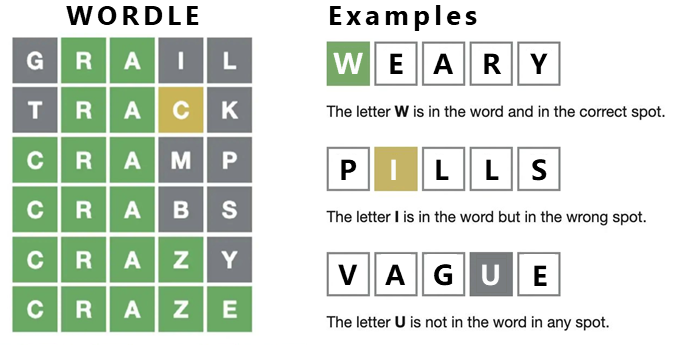
\includegraphics[scale=0.6]{wordle_comb.PNG} \label{1}
    }
    \subfigure[Report for Jul 20,2022\upcite{2}]{
    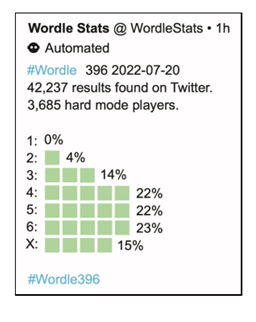
\includegraphics[scale=0.65]{wordle_comb2.png} \label{2} 
    }
    %\setlength{\abovecaptionskip}{0.1cm}
    \caption{Background Brief of Wordle}
\end{figure}


To better analyze users' scores, MCM generated daily reports from January 7 to December 31, 2022, including the date, contest number, word of the day, the number of people reporting scores that day, the number of players on hard mode, and the percentage of times players spent guessing the word. 
The example in Figure 1(b) was the distribution of reported results for July 20, 2022.

%\begin{figure}[H]
 %   \centering
 %   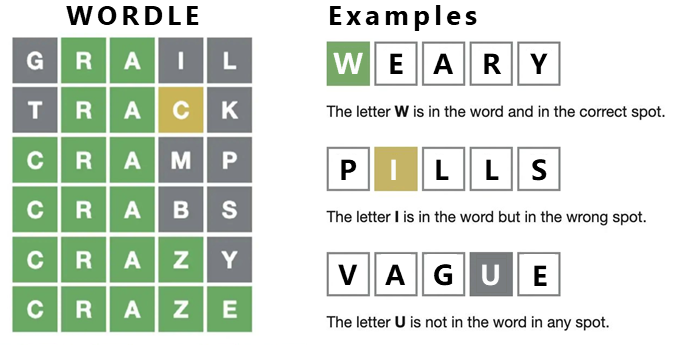
\includegraphics[scale=0.55]{wordle_comb.PNG}
 %   \caption{The rules of Wordle}
    %\label{问题二虚拟数据峰高比1-9散点图}
%\end{figure}
%调整图片与上文的垂直距离

%Figure 1: shows a schematic diagram of a wave energy device consisting of a float, an oscillator, a central shaft, and an energy output system (PTO, including a spring and a damper). (spring and damper). The oscillator, center shaft and PTO are sealed inside the float, which consists of a cylindrical shell with uniform mass distribution and a conical shell.


\subsection{Restatement of the Problem}

\begin{itemize}
	\item The number of reported results vary daily. Develop a model to explain this variation and
    create a prediction interval for the number of reported results on March
    1, 2023. Analyze how certain attributes of the word affect the percentage of scores reported that were
    played in hard mode.
    \item For a given future solution word on a future date, develop a model to predict the distribution of the reported results and analyze the uncertainties of the model and predictions.
    Then give a specific example of the prediction for the word
    EERIE on March 1, 2023. Analyze the credibility of the prediction result.
    \item Develop a model to classify solution words by difficulty. Identify the
    attributes of a given word that are associated with each classification. Then classify the example word EERIE and discuss the accuracy of the classification model. 
    \item List and describe some other interesting features of this data set.
\end{itemize}
	
%\begin{itemize}
%	\item Problem 1 is to model the motion of the float and the oscillator, discuss and solve for the first 40 wave cycles with time intervals of The displacement and velocity of the vertical oscillation at an interval of 0.2s. Since the float is subjected to linear periodic micro-amplitude waves, the sea level height can be approximated as The float and the oscillator motion are described quantitatively by taking the sea level position as the zero point and the vertical direction as the positive direction to establish the coordinate axis. The quantified description of the motion of the float and the oscillator is done. Combining with the data in Appendix 3 and 4, the force analysis of the float and the oscillator is carried out separately, and the differential equations describing the position of the float and the oscillator are obtained. The first-order explicit differential equations are obtained by permutation. Then, we use the odefun function in matlab to solve the differential equations. The numerical solution of the differential equation is solved by using the odefun function in matlab to obtain the displacement and velocity of the pendular oscillator at the requested time.

%	\item Two cases of damping coefficients are given in Problem 2, and the maximum output power of the PTO system and the corresponding optimal damping coefficient are to be solved separately. The optimal damping factor. Firstly, the mathematical model is constructed based on the expression of the average power to obtain the average power as a function of the damping coefficient in the first question, and the average power as a function of the scale factor and power exponent in the second question. In the first question, the average power is obtained as a function of the damping coefficient, and in the second question, the average power is obtained as a function of the scale factor and power exponent. For a given step size, the independent variables of the two functions are The scatter plot of the average power is obtained by traversing the independent variables of the two functions in the interval. Observing the data distribution in the scatter plot, the The maximum points are retrieved and estimated to obtain the maximum average output power and the corresponding damping coefficient.

%	\item Problem 3 is to model the motion of float and oscillator pendulum longitudinal rocking, and solve for the pendulum displacement, pendulum velocity, longitudinal rocking angular displacement, and longitudinal rocking angular velocity for a time interval of 0.2s during the first 40 wave cycles. The pendular displacement, pendular velocity, longitudinal displacement, and longitudinal velocity of the float and oscillator for the first 40 wave periods with 0.2s interval are solved. Firstly, we assume the motion of the float rotation axis and its axis center. The data in Annex 3 and 4 are combined to analyze the forces on the float and the oscillator in the direction of vertical oscillation and the direction of longitudinal oscillation. The kinematic differential equations of the float and the oscillator are then listed according to Newton's second law and transformed into first-order explicit differential equations by permutation. equations. The numerical solution of the differential equation is solved by using the odefun function in matlab to obtain the relevant data at the requested time.

%	\item Problem 4 is to solve for the maximum average output power and the corresponding damping factor for the given parameter range based on the model of Problem 3. damping coefficient. Firstly, we use the parameters in the annex to solve for the relative displacement and relative velocity during the longitudinal rocking of the pendulum for the given linear and rotational damping coefficients.The relative displacement and relative velocity of the longitudinal rocking process with the given linear and rotational damping coefficients. The modeling idea is the same as Problem 2, and then the numerical model of the average output power is constructed. Due to the direct The maximum average power point is solved by the multiple search method because of the high time cost of direct high-density search. Step by step After narrowing the interval and step size to achieve a certain accuracy, the maximum value of the average output power and its corresponding optimal damping coefficient are obtained.

%\end{itemize}


\subsection{Our Work}

We totally built four models to solve the problems. They are ARIMA Model for problem 1.1, Linear Fitting Model for problem 1.2, Regression Analysis Model for problem 2, and Decision Analysis Model for problem 3. 
We implemented all models with the programs and analyzed the results in a comprehensive manner.
Our work mainly includes the following:
\begin{figure}[H]
    \centering
    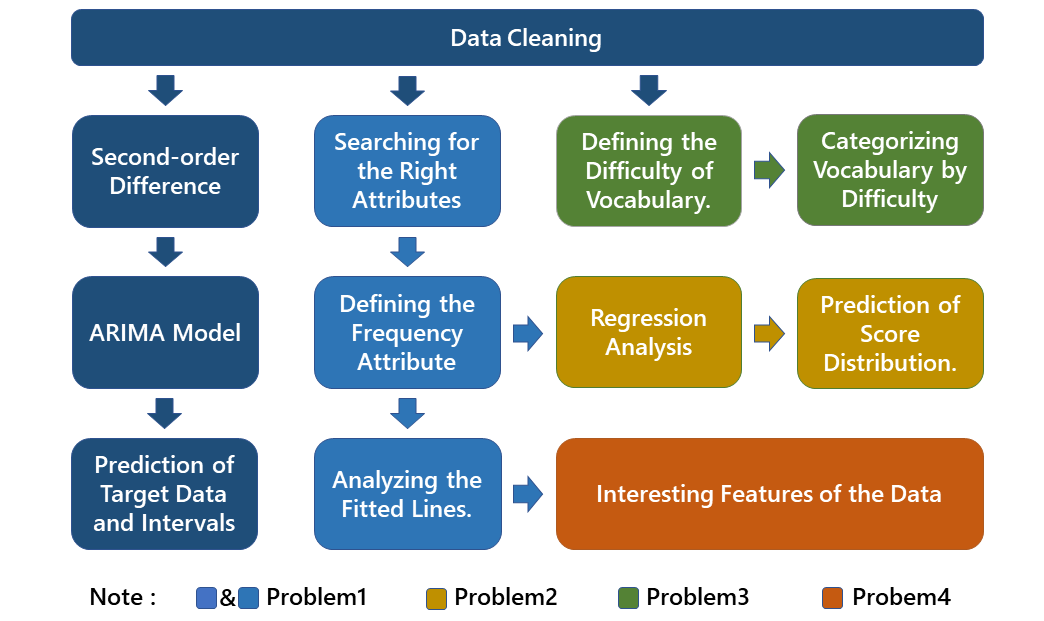
\includegraphics[scale=0.6]{overview.png}
    \caption{Model Overview}
    %\label{问题二虚拟数据峰高比1-9散点图}
\end{figure}
%\begin{itemize}
%	\item Based on the historical data of ocean temperature, a prediction model of ocean temperature is established;
%    \item The probability distribution of fish migration is given and the influence of randomness on the model is considered;
%    \item Based on the economic benefit model of fishing companies, this article evaluates the benefits of various fishing strategies under the background of fish migration and gives reasonable suggestions for the improvement of them.
%\end{itemize}




%%%%%%%%%%%%%%或者制作流程图于此%%%%%%%%%%%%%%%%



\section{Assumptions and Justifications}

\begin{itemize}%enumerate
	\item \textbf{Assumption 1: }Wordle always works smoothly and well.    \\[1pt]
    \textbf{Justification:} For the sake of authenticity, we do not exclude that Wordle has problems on some days (bad points in known data). But we assume that most of the time, especially in the future, it always works smoothly and well.
    Only a good and stable operation of Wordle can guarantee the reasonableness of known data and the predictability of future data.
    
    \item \textbf{Assumption 2: }Each person's word-guessing strategy remains the same.    \\[1pt]
    \textbf{Justification:} If the user's word-guessing strategy changes, the results will be mixed with subjective factors and not only influenced by the words. Our predictions will be unscientific. Therefore, we assume that the users' guessing strategies remain unchanged.

    \item \textbf{Assumption 3: }The frequency of people using five-letter words does not change with time.\\[1pt]
        \textbf{Justification:} If the frequency of a five-letter word is constant, the frequency of the letters in the five positions is also constant. Then we can consider frequency as a property of a word and classify words by some criteria.
    %    \item \textbf{Assumption 4: }The score percentages are accurate.\\[1pt]
    %    \textbf{Justification:} If the user's word-guessing strategy changes, the results will be mixed with subjective factors and not only influenced by the words. Our predictions will be unscientific. Therefore, we assume that the users' guessing strategies remain unchanged.

\end{itemize}

%\section{Notations}
%\begin{table}[h]
%	\begin{center}
 %       %\setlength{\tabcolsep}{12mm}{ %调整表格横向宽度
%		\begin{tabular}{ccc}
%			\toprule[1.5pt]
%			Symbol&Definition&Unit\\
%			\midrule[1pt]
%			\(x_i\)&Evaluation indicator&m\\
%			\({\tilde x_i}\)&Standardized indicators&m\\
%			\({R}\)&Correlation coefficient matrix&m\\
%			\(y_i\)&Principal Components&m\\
%			\(b_i\)&The information contribution of eigenvalue&m\\
%			\(T\)&Composite score&m\\
%			\bottomrule[1.5pt]
%		\end{tabular}%}
 %       \caption{Notations}
%	\end{center}
%\end{table}


%%%%%%%%%%%%%%%%%%%%%%%%%%%%%%%%%%%%%%%%%%%%

\section{Problem I: Number Prediction and Attribute Analysis }

\subsection{Time Series Forecasting Model}
\subsubsection{Data Cleaning}
The attached data file, like most real-world datasets, may contain some data entry errors. 
Since the number of reported results varies roughly according to some pattern, we use a third-order polynomial to fit the data and remove bad points by analyzing the residuals.
We numbered the dates in the data from smallest to largest as the $a_3$ axis. Extract the number of reported results and the number in hard mode as $a_1$ and $a_2$ axes. The fitting results are shown in Figure 3.
\begin{figure}[H]
    \centering
    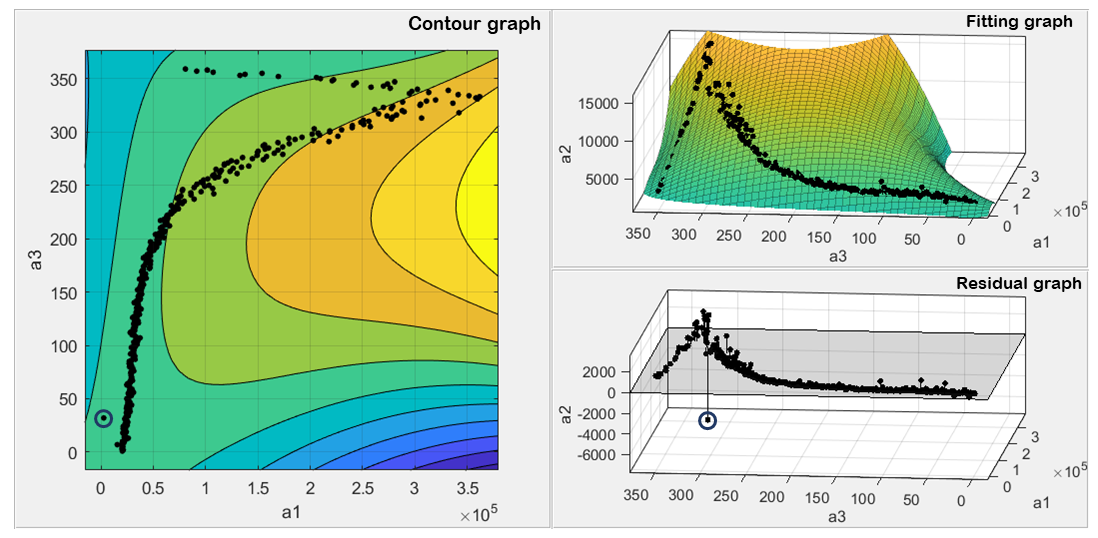
\includegraphics[scale=0.53]{1_1datafit.png}
    \caption{Polynomial Fitting and Residual Distribution}
    %\label{问题二虚拟数据峰高比1-9散点图}
\end{figure}%修改图例,标注坏点
By fitting, we excluded the outlier points $\#529$ and $\#239$ (marked with circles in Figure 3).
At the same time, we compared the attached words with the dictionary data\upcite{3} (by python) and excluded four-letter words and words not considered as words from the data. 
To ensure that the remaining amount of data is still representative, we totally cleaned out 5 bad points from 359 sets of data, accounting for $1.4\%$.
The data we cleaned out are shown in Table 1.
\begin{table}[h]
	\begin{center}
       \setlength{\tabcolsep}{11mm}{ %调整表格横向宽度
		\begin{tabular}{ccc}
			\toprule[1.5pt]
			Contet Number&Word&Reason\\
			\midrule[1pt]
			239&study&Fitting anomaly\\
            314&clen&Four letters\\
            473&marxh&Not a word\\
            525&tash&Four letters\\
            529&robin&Fitting anomaly\\
			\bottomrule[1.5pt]
		\end{tabular}}
        \caption{The Data Cleaned Out}
	\end{center}
\end{table}

%去除坏点即理由(范文1)
    %多种清洗数据的手段:1.两个四字词 2.marxh无这个词 3.naive 4.两个怪点
\subsubsection{Model Building}
It can be seen from Figure 1 that the total number of reported results roughly tends to increase and then decrease as the data time progresses, which is a non-stationary and trending series. Therefore, we use the method of non-stationary time series analysis to build the prediction model.

%二、三阶差分可以较好地描述曲线趋势
\begin{itemize}
    \setlength{\parskip}{0.2pt}
	\item \textbf{Second-order Difference}\\
	Since the number of reported results varies curvilinearly over time, we use a second-order difference model to extract the effect of curvilinear trends. Although higher-order differences theoretically work better, given the amount of data in this problem, they will also result in the loss of data points. Therefore, we use second-order difference.\\
    Set the reported results as $x_1,x_2,\cdots,x_n$, then the second-order difference is
    \begin{equation}    
    \Delta^{2} x_{i}=\sum_{j=0}^{2}(-1)^{j} C_{2}^{j} x_{i-j}
    \end{equation}
    
    \item \textbf{ARIMA Model}\\
    Autoregressive integrated moving average model (ARIMA model) is one of the time series forecasting analysis methods.
    In ARIMA (p, d, q), p, q, d each refers to the number of autoregressive terms, the number of sliding average terms, and the number of differences (orders) made to make it a smooth series. 
    Thanks to convenient python, we can directly use the statsmodels library in python for time series prediction.
    
    \item \textbf{Confidence Interval}\\
    We use the arima model to obtain the predicted value$ x_i'$ for the known data point $x_i$.
    Set the number of known data as $n$. Then the variance of the regression is
    \begin{equation}   
    \sigma^{2}=\frac{\sum(x_i-x_i')^{2}}{n}
    \end{equation}
    Set the number to be predicted as $x_p$, then the confidence interval of $x_p$ is
    $x_p \pm {z}_{\alpha / 2} \frac{\sigma}{\sqrt{n}}$.\\
    Here, we can specify $\alpha = 0.05, z_{0.025}=1.96$, which represents a $95\%$ confidence level.

\end{itemize}

In summary, we built an ARIMA model with second-order differences. 
Given that the number of reported results were too large, we took logarithm of the data with a base of ten, in order to reduce the effect of large fluctuations in the data . After obtaining the predicted data and the prediction interval, the data were permuted exponentially. 
The model flow is shown in Figure 4.

\begin{figure}[H]
    \centering
    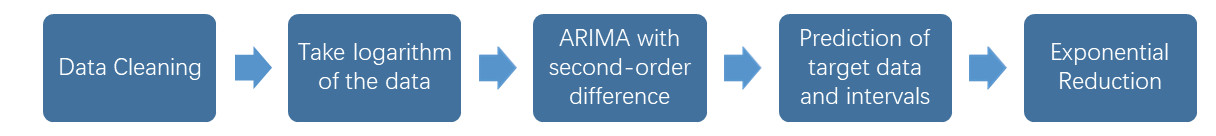
\includegraphics[scale=0.5]{1_1 flow2.png}
    \caption{Time Series Analysis Flowchart}
\end{figure}




\subsubsection{Results and Analysis}
We implemented the model 3.1.2 programmatically (see Appendix for details). By plotting the actual values against the predicted values in the original date (as shown in Figure 5(a)), we found that our prediction works well for the known data. We also plotted all the predicted points within the original date and forecast date (as shown in Figure 5(b)), and it can be found that the number of our prediction is in accordance with the original data variation pattern.

\vspace{-0.2cm} 
\begin{figure}[htbp]
   \centering
    \subfigure[Graph of Original Versus Predicted Values]{
    %原始日期内,对数
    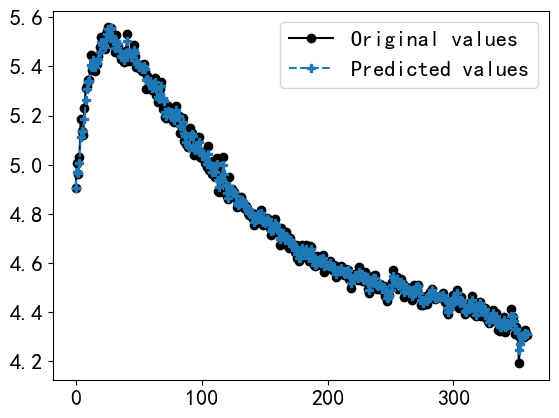
\includegraphics[scale=0.5]{1_1results21.png} \label{1}
    }
    \subfigure[Graph of Predicted Data]{
    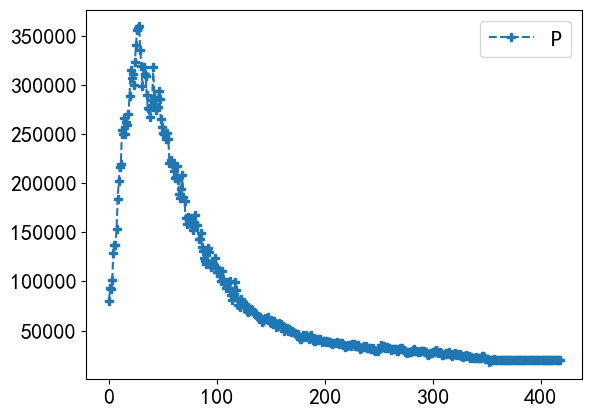
\includegraphics[scale=0.5]{1_1results22.png} \label{2} 
    }
    %\setlength{\abovecaptionskip}{0.cm}
    \caption{Prediction Results of ARIMA Model}
\end{figure}

However , we still cannot assert that the prediction is accurate. To ensure the scientific validity of the prediction, we need to further analyze some indicators of the model (as shown in Figure 6).

\begin{figure}[H]
    \centering
    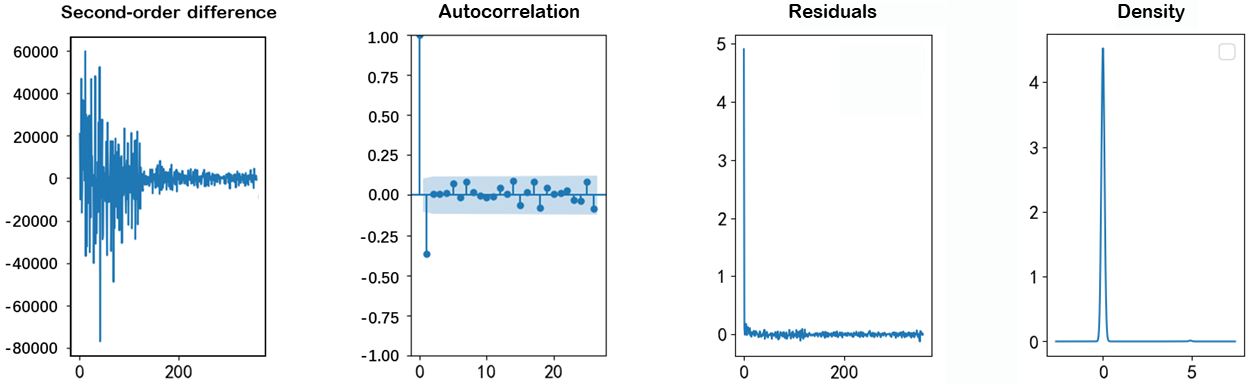
\includegraphics[scale=0.49]{1_1results.png}
    \caption{Indicators of ARIMA model}
\end{figure}

\begin{itemize}
%\setlength{\itemsep}{0pt}
%\setlength{\parsep}{0pt}
\setlength{\parskip}{0pt}
	\item \textbf{Autocorrelation:} The autocorrelations are almost all below 0.15, indicating that the existence of autocorrelation between the random error terms is weak and the model prediction is good.
    \item \textbf{Residuals:} The points on the residual plots are distributed around 0, random and irregular, indicating that the predictions are stable and accurate.
\end{itemize}
\vspace{-0.2cm} 

In addition, the images of \textbf{Second-order difference} and \textbf{Density} are both normal. Therefore, we can declare that the prediction is relatively scientific and accurate.
Our prediction for March 1, 2023 is shown in Table 2. The prediction interval has a $95\%$ confidence level. The predicted number is not in the center of the interval because we performed a logarithmic operation. 
\begin{table}[h]
	\begin{center}
       \setlength{\tabcolsep}{11mm}{ %调整表格横向宽度
		\begin{tabular}{|c|c|c|}
			\toprule[1.5pt]
			Tries&Predicted Number&Predicted Interval\\
			\midrule[1pt]
			March 1, 2023&20564&[17480, 24191]\\
            \bottomrule[1.5pt]
		\end{tabular}}
        \caption{Conclusion of Problem 1-1}
	\end{center}
\end{table}
%结果,置信区间
%\subsubsection{Sensitivity Analysis}
 %加噪声处理
%%%%%%%%%%%%%%%%%%%%%%%%%%%%%%%%%%%%%
\subsection{Linear Fit Analysis Model}

\subsubsection{Model Building}

\begin{enumerate}
    %\setlength{\itemsep}{0pt}
    %\setlength{\parsep}{0pt}
    %\setlength{\parskip}{0pt}
        \item \textbf{Stats the Frequency of Word Usage} \\
        We retrieved data for the five-letter alphabet\upcite{3} and obtained the frequency of use of all letters in each position. Then we normalized the frequency data.
        Set $\alpha$ as the i-th of the five letters, and its frequency is denoted as $f(\alpha,i)$.
        \item \textbf{Sets the Indicator of the Attributes} \\
        For a given five-letter word $\alpha_1\alpha_2\alpha_3\alpha_4\alpha_5$, define its frequency attribute as 
        \begin{equation}
           L(\alpha_1\alpha_2\alpha_3\alpha_4\alpha_5)=-lg(f(\alpha_1,1))-lg(f(\alpha_2,2))-lg(f(\alpha_3,3))-lg(f(\alpha_4,4))-lg(f(\alpha_5,5))
        \end{equation}
        For example, the frequency attribute of 'words' is defined as
        \begin{equation}
            L(words)=-lg(f(w,1))-lg(f(o,2))-lg(f(r,3))-lg(f(d,4))-lg(f(s,5))
        \end{equation}
        The larger the $L(\alpha_1\alpha_2\alpha_3\alpha_4\alpha_5)$, the less frequently the word appears.
        \item \textbf{Fit the Scatter Plots} \\
        Plot scatter plots for different number of attempts versus frequency attributes $L$. Observe the distribution pattern of the images and describe the variation by fitting the data.
\end{enumerate}

\subsubsection{Results and Analysis}
We implemented model 3.2.1 programmatically and fitted the scatter plots (see Appendix for details).
The fitting plots are shown in Figure 7.

\begin{figure}[H]
    \centering
    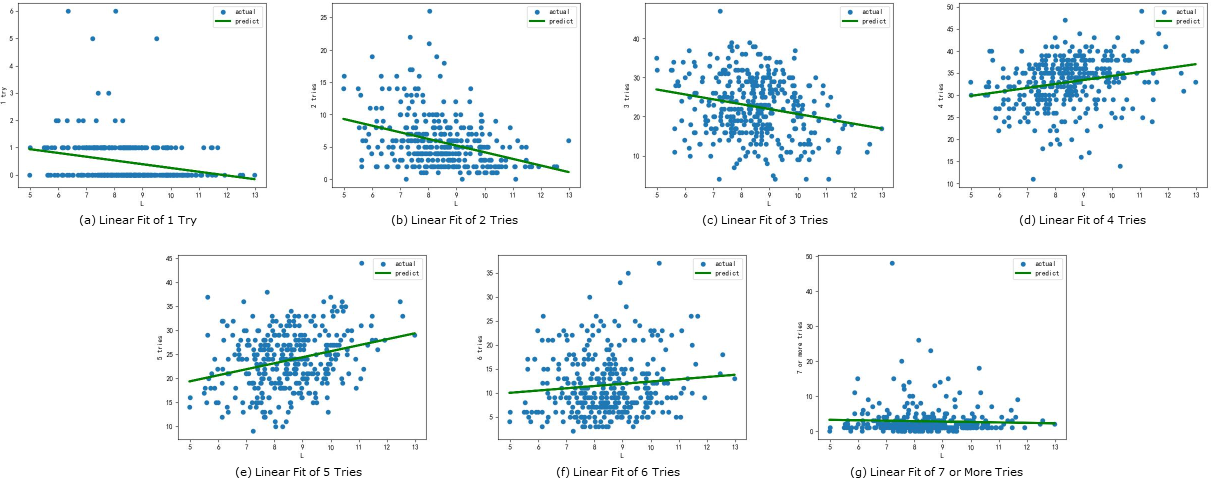
\includegraphics[scale=0.53]{1_2.png}
    \caption{Scoring Percentage Fitting Graph}
\end{figure}

It is worth noting that the fit we use here is not to show how good the correlation coefficients are, but to present a more intuitive picture of the distribution pattern of the scattered data.
As we can see in Figure 7, except for Figure 7(a), the rest of the scatters have a tendency to aggregate.
This means that there is a correlation between the percentage distribution of the number of attempts and the frequency attribute $L$, and the linear fit can help us to better recognize their relationship.

%\begin{table}[h]
%	\begin{center}
 %      \setlength{\tabcolsep}{11mm}{ %调整表格横向宽度
%		\begin{tabular}{|c|c|c|}
%			\toprule[1.5pt]
%			Date&Slope&intercept\\
%%			1& -0.138&1.630 \\
  %          2& -1.028& 14.446\\
   %         3& -1.250& 33.195\\
    %       4& 0.987& 25.367\\
     %       5& 1.251&13.152 \\
      %      6&0.470 &7.653 \\
       %     7 or more& -0.123& 3.862\\
        %    \bottomrule[1.5pt]
		%\end{tabular}}
       % \caption{Conclusion of Problem 1-1}
%	\end{center}
%\end{table}

Then we can analyze the slope of the fitted lines. The slopes of Fig. 7(a)(b)(c) are negative, while the slopes of Fig. 7(d)(e)(f) are positive. The slope of Figure 7(g) is also negative, but very close to 0. Thus, we can conclude that \textbf{as the frequency of word usage decreases, 
the frequency attribute $L$ increases, and the number of user attempts becomes roughly more.}

In addition, we also tried other attributes of words, such as the number of vowel letters, the number of repeated letters, lexical categories of words, and so on. However, the distribution of the scatterplot is rather random and there is no clear trend. 
We also tried to train machine learning models to classify words by attributes, but unfortunately the test results were not good either. In the process of mining the data attributes, \textbf{we found some interesting phenomena of the data, as shown in Section 6.}





%%%%%%%%%%%%%%%%%%%%%%%%%%%%%%%%%%%%%%%%%%

\section{Problem II: Score Distribution Prediction}

\subsection{Model Building}

From questions 1-2, we found a strong correlation between the percentage of scores and the usage frequency of each letter in a five-letter word. 
However, after creating the relevant graphs, we found that the percentage of scores did not correlate strongly with the usage frequency of the letter at a certain position, and the distribution was quite scattered. 
After comparing, we decided to use a regression tree model to portray the relationship between the usage frequency of letters and the percentage of scores.
\subsubsection{Regression Tree Model}

To clarify the theory of regression trees, we use Figure 8 as an example.


\begin{figure}[htbp]
    \centering
     \subfigure[Regression Tree Divides the Plane.]{
     %原始日期内,对数
     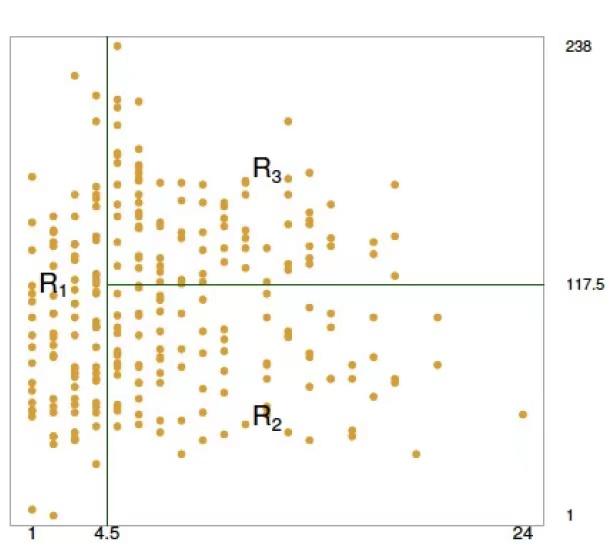
\includegraphics[scale=0.34]{2_01.jpg} \label{1}
     }
     \subfigure[Regression Tree Divides a Section Again.]{
     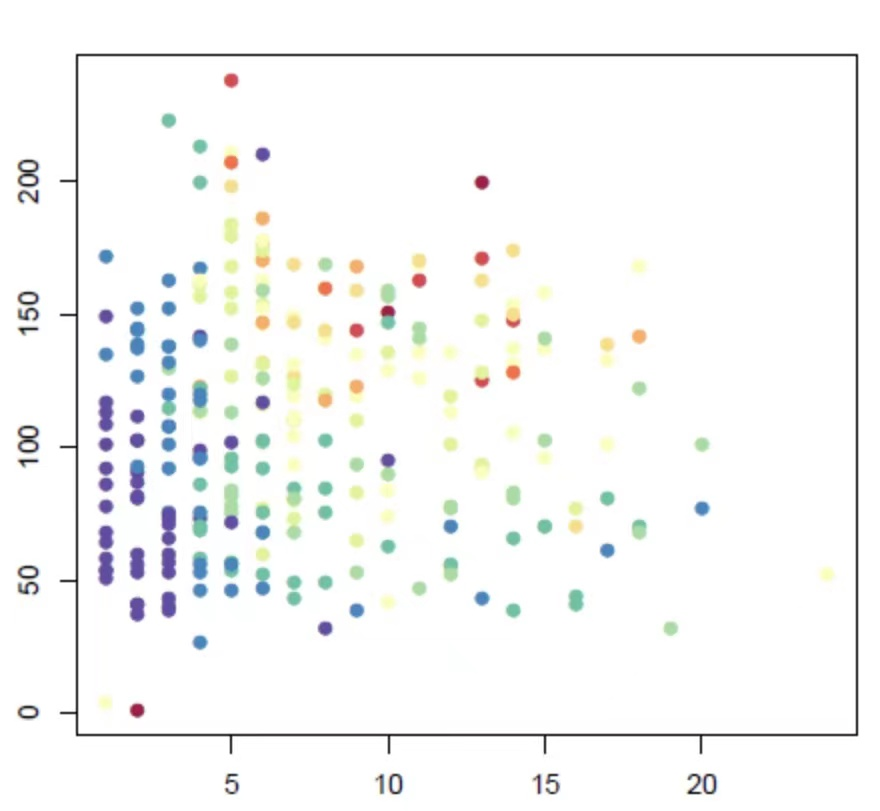
\includegraphics[scale=0.228]{2_02.jpg} \label{2} 
     }
     %\setlength{\abovecaptionskip}{0.cm}
     \caption{Principle of Regression Tree}
 \end{figure}

In the example of the data below, the horizontal and vertical coordinates each represent a feature, and the color of the point represents the result corresponding to the feature there.
The regression tree divides the plane into sections, and for samples within that section, the results are averaged over the region. 
As a result, we have got a simple classification prediction.
For each divided section, the regression tree model continues to perform similar operations to divide the region into smaller sections. We use the average of the sample points within that part to assign values to the data there, and then we can get a prediction model for each feature of the target data.

\subsubsection{Boosting Model}


The Adaboost classification model is equivalent to a forward-distributed additive model with an exponential loss function.
    The model $f_{k+1}$ obtained from the $(k+1)$th round of training can be expressed as
    \begin{equation}
    f_{k+1}(x) = f_{k}(x) + \alpha_{k+1}g_{k+1}(x).
    \end{equation}
    
    $g_{k+1}(x)$ is our trained weak regression function, namely the weak regression tree.
    
    \begin{itemize}
        \setlength{\parskip}{0.2pt}
        \item \textbf{Optimization of Regression Tree}\\
        In dealing with the problem, the tree too small will lead to poor results, while the tree too large will lead to overfitting. Therefore, we try to use the idea of Boosting in integrated learning to enhance the regression tree instead of just deepening the tree.
       \item \textbf{Advantages of Boost Model}\\
       The Boosting algorithm integrates the properties of each layer of the weak regression function and evaluates the weighting to ensure that the model still performs well over different regions. Moreover, the boosting algorithm can make the error decrease gradually in the process of continuous iteration.
    \end{itemize}
     
    



\subsection{Results and Analysis}

We implemented the regression analysis model 4.1 with the program (see Appendix for details).
By training the model with the usage frequency of each letter, we finally got the prediction graphs shown in Figure 9.
(The original data are represented by yellow dots and the predicted data are represented by green dots.)

\begin{figure}[H]
    \centering
    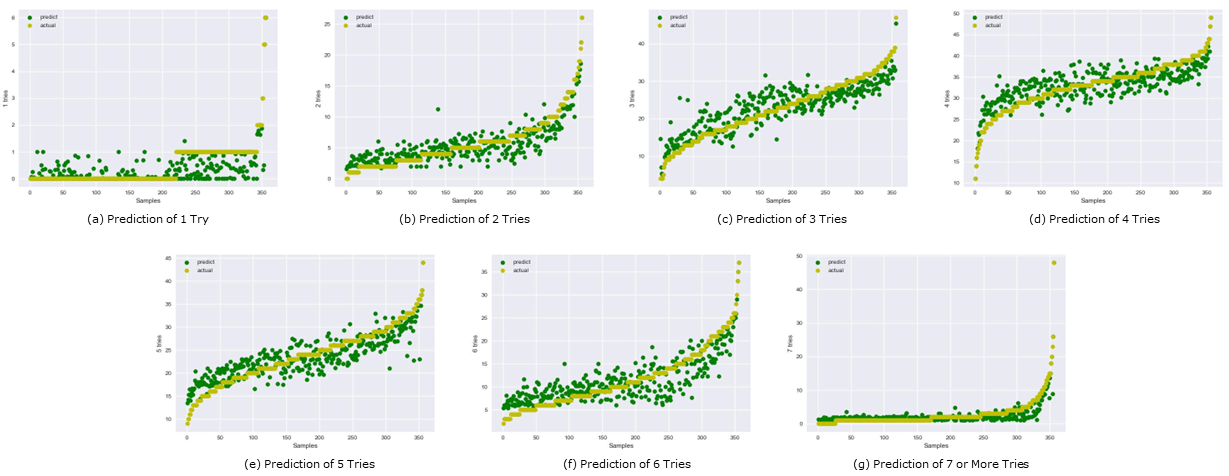
\includegraphics[scale=0.52]{2_2.png}
    \caption{Predicted Scoring Percentage Distribution Graph}
\end{figure}

The images show that the predicted data points are roughly distributed around the original data, so the prediction results are relatively good. 
According to the letter frequency table\upcite{3}, we found out the letter frequency corresponding to 'Errie' and substitute it into the model operation. The prediction results obtained are shown in Figure 10.

\begin{figure}[H]
    \centering
    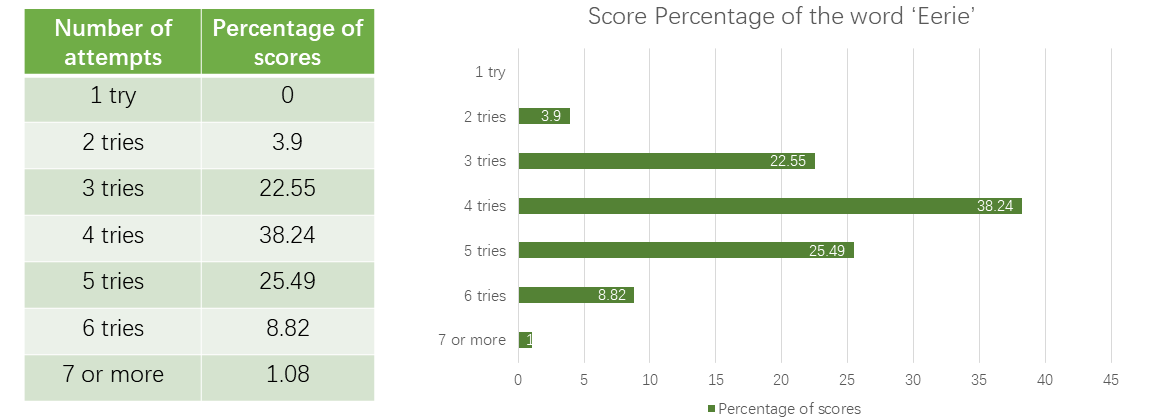
\includegraphics[scale=0.52]{2_3.png}
    \caption{Prediction of the Score Percentage of Eerie  }
\end{figure}

However, we still cannot ignore the gap between the predicted points and the original points. Although we tried to make improvements to the algorithm and also tried to replace the indicators for training, the prediction points never matched the original points perfectly. This may be because the indicator mining is not deep enough, the training set is too small, or the data is not representative enough. The larger the data set is, the more comprehensive the indicators we know, the more accurate the prediction will be.

%%%%%%%%%%%%%%%%%%%%%%%%%%%%%%%%%%%%%%%%%%%%%

\section{Problem III: Vocabulary Difficulty Classification}

\subsection{Model Building}

%\subsubsection{Defining Difficulty levels}

From Model 4.1, we can recognize the relationship between the frequency of using each letter in a word and the difficulty of word guessing. To measure the difficulty of guessing, we introduce the indicator $ H$. The percentage of $i$ tries for a word $p$ is noted as $y_i$.
\begin{equation}
    H(s) =100* (\sum_{i=1}^{6}iy_i+8y_7)
\end{equation}    

We consider scoring the difficulty level of $H(s)$. From Figure 11, it can be assumed that the difficulty coefficients follow a normal distribution.

\begin{figure}[H]
    \centering
    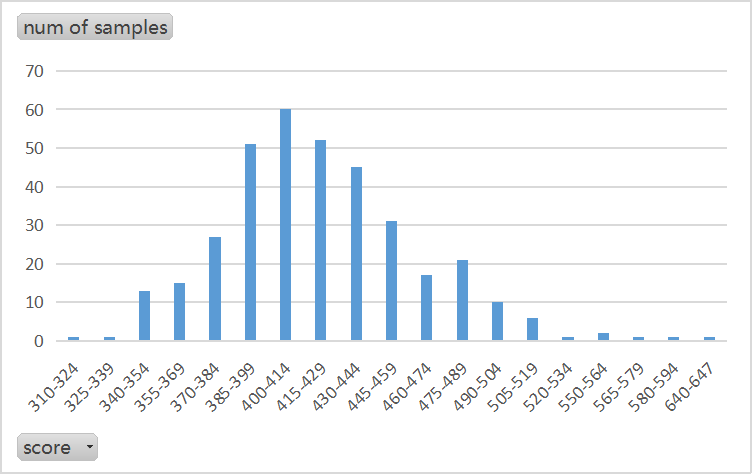
\includegraphics[scale=0.7]{3_1.png}
    \caption{Plot of the Distribution of $H(s)$ }
\end{figure}

Then, assume that there are as many words at different difficulty levels. That is, a five-letter word is randomly selected with equal probability of its difficulty level.
From the data set, we calculated the mean and standard deviation of the difficulty levels.
\begin{equation}
    \mu =422.564606741573,\enspace \sigma = 43.05951962648127
\end{equation} 

Consider four levels: very hard, hard, easy, very easy.

That is, consider the node $x_i,\enspace i = 0,1,... ,4$, such that

\begin{equation}
    \int_{x_i}^{x_i+1}\frac{1}{\sqrt{2 \pi }\sigma}e^{-\frac{(x-\mu)^2}{2\sigma^2}}  \,dx = \frac14, \enspace i = 0,1,2,3,\enspace x_0 = - \infty, x4 = \infty
\end{equation} 

Then we can get

\begin{equation}
    A = \left\{s\mid H(s) > x_3 \right\},\enspace B = \left\{s\mid x_3 \geq H(s) > x_2 \right\} 
\end{equation} 
\begin{equation}
    C = \left\{s\mid x_2 \geq H(s) > x_1 \right\}, \enspace D = \left\{s\mid x_1 \geq H(s)  \right\}
\end{equation} 
\vspace{-0.1mm}

In order to classify the words better in terms of difficulty and to obtain the relevant word attributes. We consider using \textbf{decision tree algorithm.}
Detailed reasons are shown below.
\begin{itemize}
    \setlength{\parskip}{0.2pt}
    \item The decision tree algorithm performs best on the small data sets we have (decision trees are suitable for small volumes of data).
    \item Decision trees are very simple and intuitive, allowing easy classification and prediction. 
    \item Although one decision tree is prone to overfitting, we have pruning and other means to improve generalization. Decision trees are well explained in logic.
\end{itemize}


\subsection{Results and Analysis}

Using the decision tree model 5.1, we classified the word difficulty as shown in Figure 12.

\begin{figure}[H]
    \centering
    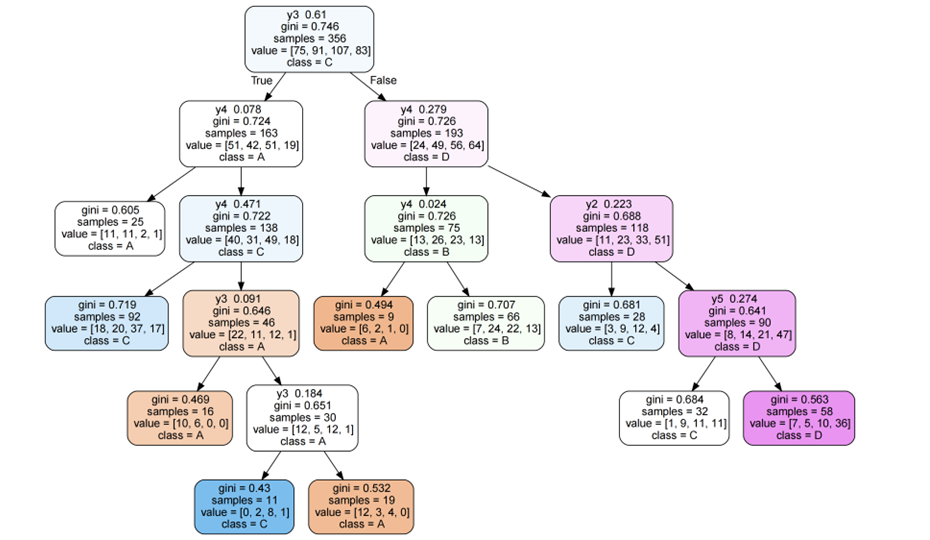
\includegraphics[scale=0.6]{3_2.png}
    \caption{Diagram of Word Difficulty Classification}
\end{figure}

\begin{itemize}
    \setlength{\parskip}{0.2pt}
    \item In the decision tree, we can see that the less frequently the letter is used, the closer the difficulty level is to A, while the more frequently the letter appears, the closer the difficulty level is to D.
    \item Particularly, the usage frequency of the third letter and the fourth letter has a greater influence on the results. It can be said that the lower the usage frequency of the third and fourth letters, higher the difficulty.
\end{itemize}


By looking up the table of letter frequencies, we got the usage frequency of letters in the corresponding positions of EERIE. We substituted the data into the model and found that \textbf{the difficulty level of EERIE is D, which is very easy}  (see Appendix for details).

From the characteristics of the words, we can see that there are many e and i. These two letters are used more frequently and have a higher probability of being guessed, so the difficulty level is naturally low.

%%%%%%%%%%%%%%%%%%%%%%%%%%%%%%%%%%%%%%%%%%%%%%
\section{Problem IV: Interesting Features of the Data Set}%other cases:Test the model
\subsection{Dare to Challenge}
In real life, when we are familiar with a certain game, we tend to try a more difficult mode. Do the data in the question show such a characteristic?
To figure this out, we calculated the daily selection rate of the hard mode, which is the number of people who selected the difficult mode divided by the total number of people. Then we fit it with the sigmoid function in matlab. The result is shown in Figure 13.
\begin{figure}[htbp]
    \centering
     \subfigure[Graph of the fitting curve]{
     %原始日期内,对数
     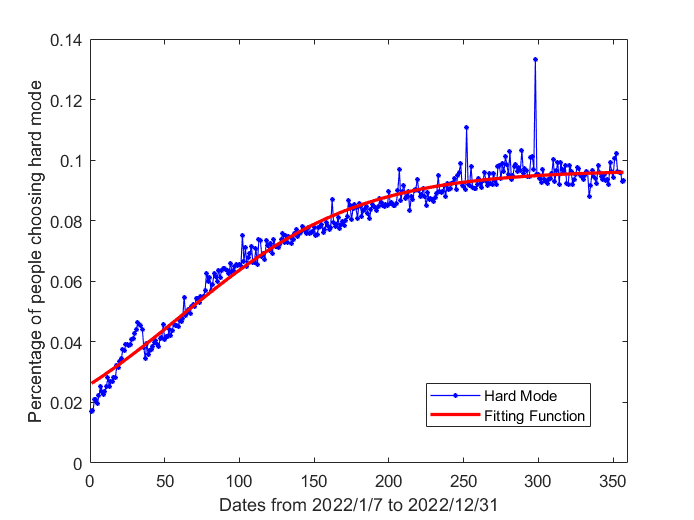
\includegraphics[scale=0.45]{4_1.png} \label{1}
     }
     \subfigure[Parameters of the Fit]{
     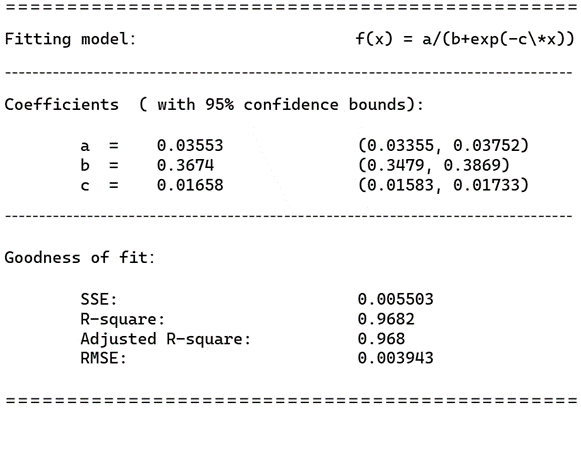
\includegraphics[scale=0.49]{4_2.png} \label{2} 
     }
     %\setlength{\abovecaptionskip}{0.cm}
     \caption{Fitting graph of the percentage of people choosing the hard mode as the date increases}
 \end{figure}

 The fit is quite good. From the graph we can see that \textbf{the daily rate of choosing hard mode increases with time roughly in the form of $e^{\frac{1}{x}}$.}




 \subsection{Common not Always Right}

We invoked the daily usage frequency lookup function WordFrequencyData from the wolfram library to sort the 356 valid data in the table from smallest to largest usage frequency. 
Then we were surprised to find that the percentage of difficulty mode scores was approximately even
(As shown in Figure 14).
Therefore, it was concluded that \textbf{the frequency of daily use of the answer words had little effect on the distribution of scores on the day.}
(Interestingly enough, the conclusion does not match our intuition. In our view, it seems that the more commonly used words are easier to guess.)

\begin{figure}[htbp]
	\centering
	\begin{minipage}{0.495\linewidth}
		\centering
		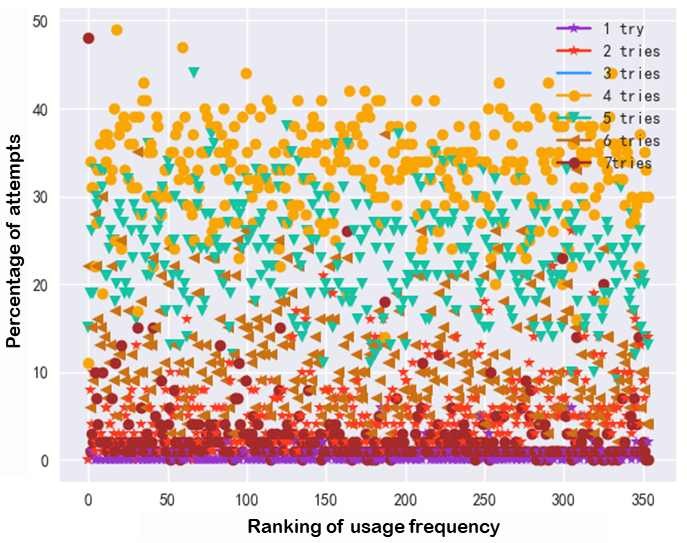
\includegraphics[width=0.9\linewidth]{4_3.png}
		\caption{Percentage versus Frequency}
    \end{minipage}
	%\qquad
	\begin{minipage}{0.47\linewidth}
		\centering
		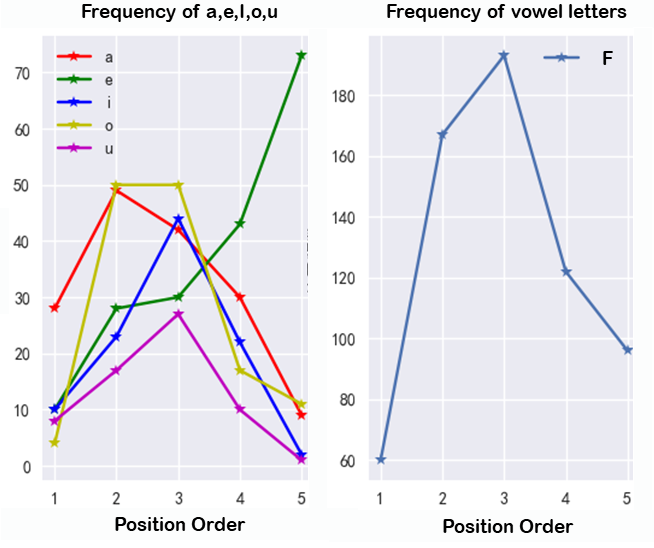
\includegraphics[width=0.9\linewidth]{4_4.png}
		\caption{Distribution of Vowel Letters}
	\end{minipage}
\end{figure}


\subsection{Where the Vowel Letters are }
We counted the distribution of vowel letters in the data words and made the following findings.
(As shown in Figure 15)
\begin{itemize}
    % \setlength{\parskip}{0.2pt}
     \item A,i,o,u are basically distributed in 1, 2, 3 positions.
     \item The further back the position, the more often e appears.
     \item Vowel letters are mostly distributed in 2,3 positions.
\end{itemize}


%\subsection{What Happened These Days ?}


%%%%%%%%%%%%%%%%%%%%%%%%%%%%%%%%%%%%%%%%%%%5%
\section{Model Evaluation and Further Discussion}
\subsection{Strengths}
\begin{itemize}
   % \setlength{\parskip}{0.2pt}
    \item \textbf{Time Series Analysis}\\
    Time series analysis is a dynamic data processing method that focuses on the interdependence of data series.
    The number of reports is closely related to the proximity of the day to the release date and the data from previous reports, so time series analysis is a very convincing model.
    \item \textbf{ARIMA Model}\\
    The ARIMA model is generally used when there are more than 50 observations. For non-stationary time series, the observed time series should be first differenced and transformed into a stationary time series.  The reported volume of Wordle has gradually leveled off with the increase of time, so using time series analysis model is a good forecasting model.
    \item \textbf{Regression Tree Model}\\
    Through the data analysis, we found that the daily scores have a great correlation with the difficulty, so by classifying the difficulty before making predictions, we unified problem 2 and problem 3 into one model.
    For small data sets, we cannot fit the relationship between input and output by neural network and machine learning, and it is also difficult to classify the difficulty of words.
    Therefore, it is ideal to classify five-letter words into ABCD classes through a decision tree model, and the average result within each class is used as the prediction value for that class.
    \item \textbf{Boosting Model}\\
    The Boosting algorithm integrates the properties of each layer of the weak regression function and evaluates the weights, which ensure that the model still performs well on different regions. Moreover, the boosting algorithm can make the errors decrease gradually in the process of continuous iteration.
\end{itemize}


\subsection{Weaknesses}

\begin{itemize}
    \item \textbf{Errors of ARIMA}\\
    The reported results of Wordle has a very high peak, which increases the difficulty of smoothing near the peak, and the ARIMA model will be affected to some extent.
    \item \textbf{Errors of Regression Tree }\\
    Since the dataset is not very informative, in the process of finding the attributes of words, we found that many attributes have no obvious trend in correlation with the percentage of scores itself, so the prediction bias would be quite large if the accurate function is obtained by function fitting or neural network calculation. Therefore, we selected the frequency of different letters appearing in different positions as attributes, and the difficulty division was not fine enough to make only a more rough estimate.

    At the same time, words of the type 'eerie' are relatively rare, and the number of words like this in the data set is minimal, so it may have a large chance error.
\end{itemize}





\subsection{Further Discussion}
To make the results more accurate, we can take the following steps.
\begin{itemize}
    \item Use a larger data set.
    \item Find more word-related attribute factors.
    \item Use more advanced models to determine. \\
    For example, when the amount of data is large can be fitted by neural networks.
    \item Make the type of decision tree model more detailed.

\end{itemize}

%%%%%%%%%%%%%%%%%%%%%%%%%%%%%%%%%%%%%%%%%%%
%\section{Conclusion}
%%%%%%%%%%%%%%%%%%%%%%%%%%%%%%%%%%%%%%%%%%%
\newpage
\section{The Letter to the Puzzle Editor of the New York Times}
\vspace{0.1cm} 
\noindent {Dear editor,}
\vspace{0.1cm} 

It is our honor to be invited to analyze the results of the Wordle game report. As response to your requirement, we are here pretty glad to have the opportunity to introduce our research and suggestions to you, with the hope that it may give you some insights of the future strategies.

\begin{itemize}
    %\setlength{\itemsep}{0pt}
    %\setlength{\parsep}{0pt}
    %\setlength{\parskip}{0pt}
        \item \textbf{Phenomenon:  The number of reported results is leveling off.}\\
        We used a time series model to predict the number of reported outcomes for a future period. According to our prediction, the total number of reported outcomes on March 1, 2023, is approximately 20564, which is roughly the same as the number at the end of December 2022. According to our results, we are sorry to say that the hot period of Wordle games has been over, and the total number of reported results has declined and leveled off in the region after experiencing an increase. In other words, our number of users has roughly stabilized.
   
        


        \item \textbf{Problem:  How to retain and attract more users?}
        \\
        In order to design programs to attract more users, we analyzed the data from the results reports and found an important phenomena.
        \begin{itemize}
            %\setlength{\itemsep}{0pt}
            %\setlength{\parsep}{0pt}
            %\setlength{\parskip}{0pt}
            \item \textbf{The ratio of choosing hard mode is increasing.} 
            \\
            By calculating the daily selection rate of the hard mode and fitting the data, we found that the daily rate of choosing hard mode increases with time roughly in the form of $e^{\frac{1}{x}}$.
        \end{itemize}
        %问题二结论
        Just as in real life, when we are familiar with a certain game, we tend to try a harder mode. There are more and more Wordle players to challenge the hard mode, and we need to increase the difficulty of this game.
%现象表明了什么……。为了……我们要……。


        \item \textbf{Strategy:  Use lower-frequency words (especially with letter z,q,x).}
    \\
            Considering that users always place more attention on letters than on the whole words while playing this game, we gave a new definition of the frequency of words. For a word with five letters, we focused on the logarithmic sum of the frequency of each letter in its position.
            By plotting the scatter plot of frequency versus number of attempts, we found that the lower frequency of the word, the more attempts the users make.
            By making a word frequency table, we found that the letter z,q,x occurs least frequently in the words that were guessed.
           % \item \textbf{Increase the difficulty of words.} 
%问题三筛选指标
        \item \textbf{Tool: A customized vocabulary classification and score distribution prediction tool.}\\
        We constructed a score percentage prediction model based on regression analysis and boosting algorithm, and a word difficulty classification model based on decision analysis. These models showed good results even with a small data set. We believe they will be of even greater value using the large amount of data from the New York Times.



\end{itemize}






   % \end{itemize}

 We are really appreciated for this opportunity to analyze the results of the Wordle game report, and we are convinced that our proposal can be utilized in retaining and attracting more users. Please feel free to contact us for further information on the project.


 \vspace{0.3cm} 
 \noindent {Sincerely yours}

 \vspace{0.1cm} 
 \noindent {MCM Team \#2301831}








\newpage


\begin{thebibliography}{99}
	\bibitem{1}"What is the Wordle that suddenly exploded abroad recently?"Accessed on February 18, 2023 at \url{https://blog.csdn.net/sinat_33224091/article/details/122646324}
	\bibitem{2} “Wordle Stats.” Twitter, July 20, 2022
    \bibitem{3}Word Frequency Data. Accessed on February 18, 2023 at \url{https://reference.wolfram.com/language/ref/WordFrequencyData.html}
    \bibitem{4}L. Breiman. Random forest. Machine Learning, 45:5–32, 2001.
    \bibitem{5}Jerome H. Friedman. Stochastic gradient boosting. Computational Statistics Data Analysis, 38(4):367–378, 2002.
    \bibitem{6} L. K. Hansen and P. Salamon. Neural Network Ensembles. IEEE Computer Society 1990.
    \bibitem{7}Lewis, David D, Schapire, Robert E, Callan, James P, Papka, and Ron. Training algorithms for linear text classifiers. pages 298–306, 1996.
    \bibitem{8}Dragos D. Margineantu and Thomas G. Dietterich. Pruning adaptive boosting. In Fourteenth International Conference on Machine Learning, pages 211–218, 1997.
    %\bibitem{9}
\end{thebibliography}


\newpage
\section{Appendices}
\subsection{The usage frequency table of letters we made}
\begin{figure}[H]
    \centering
    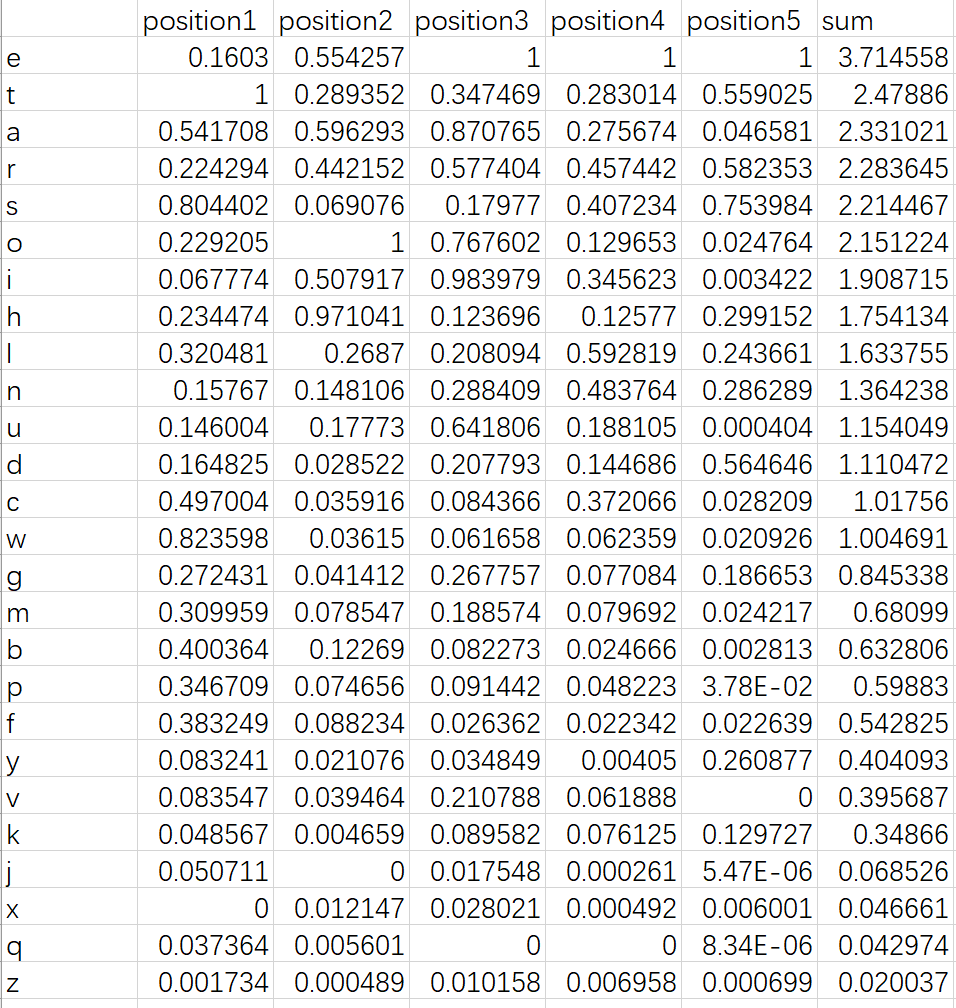
\includegraphics[scale=1.32]{and1.png}
   % \caption{Diagram of Word Difficulty Classification}
\end{figure}






\subsection{Problem 1 related codes}
\subsubsection*{Problem 1-1 ARIMA model with second-order difference}
\newpage
\begin{python}
#Question related data is stored in input3 .csv
    import pandas as pd, numpy as np
    import statsmodels.api as sm
    import matplotlib.pylab as plt
    from statsmodels.graphics.tsaplots import plot_acf, plot_pacf

    plt.rc('axes',unicode_minus=False)
    plt.rc('font',size=16); plt.rc('font',family='SimHei')
    df=pd.read_csv('input3.csv')
    plt.subplot(1,2,1); plt.plot(df.num.diff()) #Difference
    plt.title('First-order difference')
    ax2=plt.subplot(1,2,2)
    plot_acf(df.lognum.diff().dropna(), ax=ax2,title='Self-relation') 
    plt.show()

    md=sm.tsa.arima.ARIMA(df.lognum, order=(2,1,0)).fit()
    print(md.summary())

    residuals = pd.DataFrame(md.resid) #Calculate the residuals
    fig, ax = plt.subplots(1,2)
    residuals.plot(title="residuals", ax=ax[0])
    residuals.plot(kind='kde', title='Density', ax=ax[1])
    plt.legend(''); plt.ylabel('')          

    zmd=md.predict(1,359)  #Comparison of raw data and predicted values
    years=[0]
    for i in range(0,359):
        years.append(i)
    plt.figure()
    plt.plot(years[1:],df.lognum,'o-k')
    plt.plot(years[1:],zmd,'P--')
    plt.legend(('Original values','Predicted values'))
    plt.show()

    print(residuals[1:])
      
    tmd=md.predict(1,419)

    k=[tmd[419]-1.96*0.036,tmd[419]+1.96*0.036]
    print(10**tmd[419])
    print([10**k[0],10**k[1]])
    years2=[0]
    for i in range(0,419):
        years2.append(i)

    plt.figure()
    plt.plot(years2[1:],10**tmd,'P--')
    plt.legend(('Predicted value'))
    plt.show()
\end{python}

\subsubsection*{Problem 1-2 Linear Fitting and Plotting}
Figure 7 (a) as an example.
\begin{python}
#Question related data is stored in Cmcm_word_tag_sp_level11.csv
    import pandas as pd
    import matplotlib.pyplot as plt
    import pylab
    from sklearn.linear_model import LinearRegression 

    #Scatter plot of data distribution
    file=pd.read_csv("Cmcm_word_tag_sp_level11.csv")
    plt.rcParams['font.sans-serif'] = ['SimHei']  
    plt.scatter(file.iloc[:,29],file.iloc[:,22])
    plt.xlabel("L")
    plt.ylabel("7(X)try")
    pylab.show()
    print(file.iloc[:,[29,22]].corr())
    #Fitting a straight line
    model = LinearRegression() #Create linear regression objects
    x=file[['mu']] 
    y=file.t7
    model.fit(x,y) #Fitting a linear regression model

    #plot
    plt.scatter(file.mu,file.t7,label = 'actual')
    plt.plot(file.mu,model.predict(x),'g-',linewidth = 3,label = 'predict')
    plt.xlabel("L")
    plt.ylabel("7 or more tries")
    plt.legend()
    plt.savefig('7_tries.jpg')
    pylab.show()
    print("intercept and coef:",model.intercept_,model.coef_) 
    #View intercept and slope
\end{python}

\subsection{Problem 2 related codes}
Code for training.
\begin{python}
#The problem-related code is stored in try7_plot.csv
    import numpy as np
    import matplotlib.pyplot as plt
    from sklearn.ensemble import AdaBoostRegressor
    from sklearn.model_selection import train_test_split
    from sklearn.tree import DecisionTreeRegressor
    from sklearn.metrics import accuracy_score
    import pandas as pd
    #Read in data

    eerie = [[0.007272044599529789, 0.2175921813446546, 0.03569171698367764, 0.021556682611199654, 0.7491454429856049]]
    t = pd.read_csv("try7_plot.csv")
    t.describe()
    # Selecting the independent and dependent variables
    xs = t[['logy'+str(i+1) for i in range(5)]]
    y = t['t7']
    print(y)
    X_train, X_test, y_train, y_test = train_test_split(xs, y, test_size = 0.1)

    # Training data
    clf7=AdaBoostRegressor(DecisionTreeRegressor(max_depth=6), n_estimators=2000, learning_rate = 0.8, loss = "square")
    clf7.fit(X_train,y_train)

    # Model Predictions
    y_pred = clf7.predict(X_test)
    print(y_pred)
    print(y_test)
    # accuracy

    print(str(clf7.score(X_train,y_train)))
    print(str(clf7.score(X_test, y_test)))
\end{python}
Code for prediction (1 Try as an example).
\begin{python}
#Problem-related data is stored in try1_plot.csv
    x = np.linspace(1,356,356)
    t = pd.read_csv("try1_plot.csv")
    t.describe()
    # Selecting the independent and dependent variables
    xs = t[['logy'+str(i+1) for i in range(5)]]
    y = t['t1']
    y_p = clf1.predict(xm)
    print(len(y_p))
    plt.style.use('seaborn')
    plt.scatter(x,clf1.predict(xs),c='g',label = 'predict')
    plt.scatter(x,y,c='y',label = 'actual')
    plt.xlabel("Samples")
    plt.ylabel("1 tries")
    plt.legend()
    plt.savefig('1_tries_tree.jpg')
    plt.show()

    try4_eerie = clf1.predict(eerie)
    print(try4_eerie)
\end{python}

\subsection{Problem 3 related codes}
\begin{python}
#Problem-related data is stored in Cwords2.csv
    from sklearn.feature_extraction import DictVectorizer
    import csv
    from sklearn import tree
    from sklearn import preprocessing
    import numpy as np
    import pandas as pd
    import graphviz
    from sklearn.model_selection import train_test_split
    from sklearn.metrics import accuracy_score
    from sklearn.model_selection import train_test_split
    from sklearn.model_selection import GridSearchCV
    from sklearn.model_selection import cross_val_score

    file = open('Cwords2.csv', 'r')
    reader = csv.reader(file)
    headers = next(reader)
    
    featureList = []
    labelList = []
    
    for row in reader:
    labelList.append(row[10])
    rowDict = {}
    for i in range(11, 16):
        rowDict[headers[i]] = row[i]
    featureList.append(rowDict)
    file.close()

    for d in featureList:
        for x in d:
            d[x] = float(d[x])
    # Vetorize features
    vec = DictVectorizer()
    all_X = vec.fit_transform(featureList).toarray()
    # vectorize class labels
    all_y = [s for s in labelList]
    # Using decision tree for classification  
    clf = tree.DecisionTreeClassifier(criterion='gini')
    train_X, test_X, train_y, test_y = train_test_split(all_X, all_y, test_size = 0.1)
    print(test_y)
    # train the model
    clf.fit(train_X, train_y)
    # predict the test sets
    y_pred = clf.predict(test_X)

    # accuracy
    print(accuracy_score(test_y, y_pred))
    # plot
    feature_name = ['y'+str(i+1)for i in range(5)]
    dot_data = tree.export_graphviz(clf
                                    , feature_names = feature_name
                                    , class_names = ['A','B','C','D']
                                    , filled = True
                                    , rounded = True
                                )  
    graph = graphviz.Source(dot_data)
    graph

    clf = tree.DecisionTreeClassifier(max_depth=6,min_samples_leaf=5,random_state=50)
    clf         = clf.fit(all_X, all_y)  
    total_socre = clf.score(all_X,all_y)
    clf         = clf.fit(train_X, train_y)  
    train_socre = clf.score(train_X,train_y)
    print("\n========Try Model============")
    print("accuracy of the whole data sets:",total_socre)
    print("accuracy of the training sets:",train_socre)

    #-------scan the best parameters---------------------------
    clf = tree.DecisionTreeClassifier()
    param_test = {
                'max_depth':range(3,15,3)
                ,'min_samples_leaf':range(5,20,3)
                ,'random_state':range(0,100,10)
    }

    gsearch= GridSearchCV(estimator=clf,              
                    param_grid=param_test,     
                    scoring=None,         
                    n_jobs=-1,            
                    cv = 5,             
                    verbose=0            
                    )
    gsearch.fit(train_X,train_y)
    print("\n========the result of the best parameters============")
    print("the highest score of the models:",gsearch.best_score_)
    print("the best parameters of the models:",gsearch.best_params_)

    #-------train the model with the best parameters---------------------------
    clf = tree.DecisionTreeClassifier(**gsearch.best_params_)
    clf = clf.fit(all_X, all_y)  
    pruning_path = clf.cost_complexity_pruning_path(train_X, train_y)
    test_score = clf.score(test_X,test_y)     

    print("\n========training results============")
    print("number of leaves:",clf.get_n_leaves())
    print("the depth of the tree:",clf.get_depth())
    print("weighs of the features:",clf.feature_importances_)
    print("\n--------accuracy of the test:----------:\n",test_score)
    print("\n------paths of CCP---------------")
    print("ccp_alphas:",pruning_path['ccp_alphas'])
    print("impurities:",pruning_path['impurities'])

    out=[]
    for ccp_alpha1 in pruning_path["ccp_alphas"]:
        i=ccp_alpha1
        clf = tree.DecisionTreeClassifier(**gsearch.best_params_,ccp_alpha=i)
        scores = cross_val_score(clf, all_X, all_y, cv=5)
        out.append(np.mean(scores))
    print("ccp_alphas:",pruning_path['ccp_alphas'])
    print("scores:",out)

    #cut the branches
    clf =tree.DecisionTreeClassifier(max_depth=9,min_samples_leaf=8,random_state=0,ccp_alpha=0.008)

    clf = clf.fit(all_X,all_y)

    test_score = clf.score(test_X,test_y)
    print("\n==============cut the branches=====================:\n")
    print("accuracy of the test sets:",test_score)
    print("number of leaves",clf.get_n_leaves())

    #-------draw the tree-----------------------------
    dot_data = tree.export_graphviz(clf, out_file=None, 
                        feature_names=['y'+str(i+1) for i in range(5)],  
                        class_names=['A','B','C','D'],
                        filled=True, rounded=True,  
                        special_characters=True)  
    graph1 = graphviz.Source(dot_data)
    print("\n==============Decision tree after cutting branches=====================:\n")
    print("Decision tree after cutting branches")
    print(clf.predict([[0.160300414,0.554257215,0.983978652,0.457442086,1]]))
    graph1

\end{python}



%\begin{figure}[H]
 %   \centering
  %  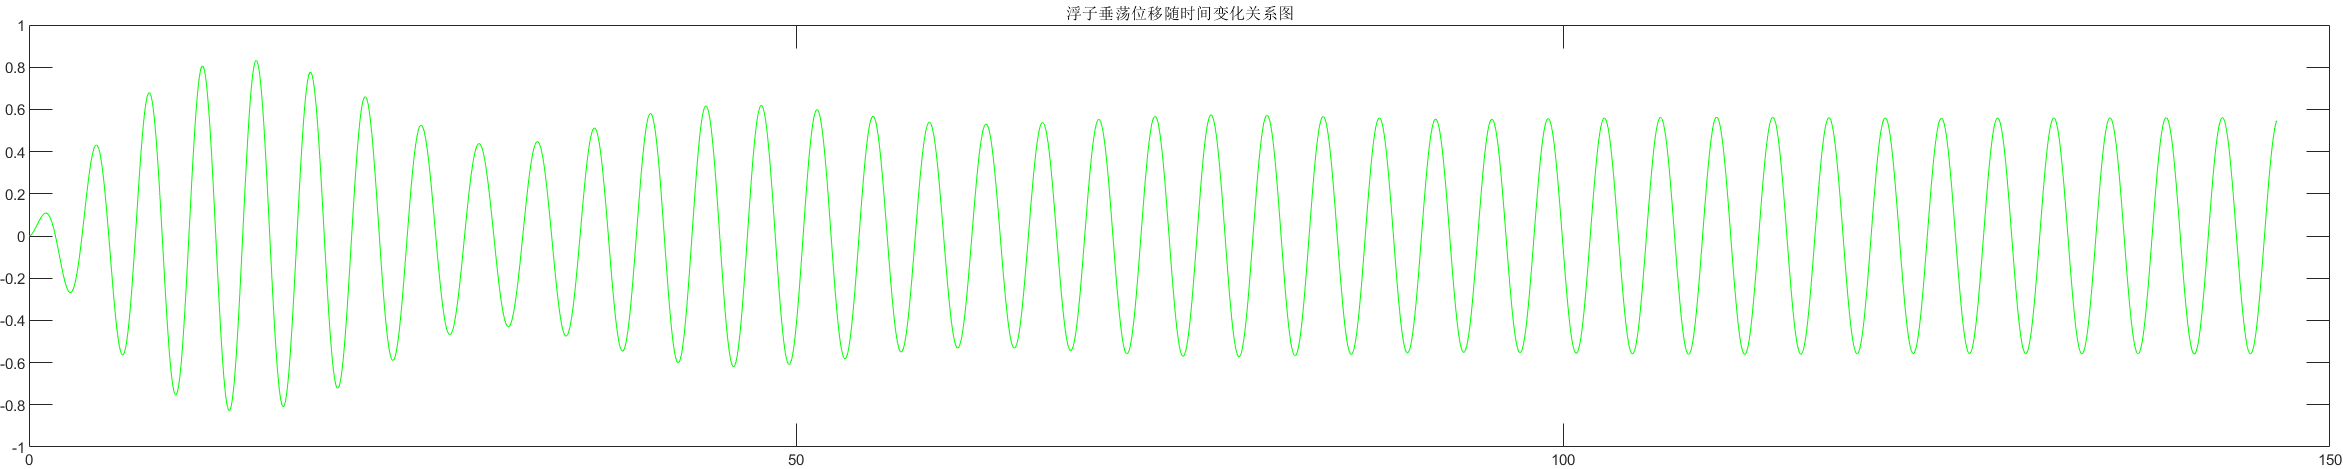
\includegraphics[scale=0.3]{问题3-1.png}
   % \caption{1}
%\end{figure}
%\begin{figure}[H]
%    \centering
 %   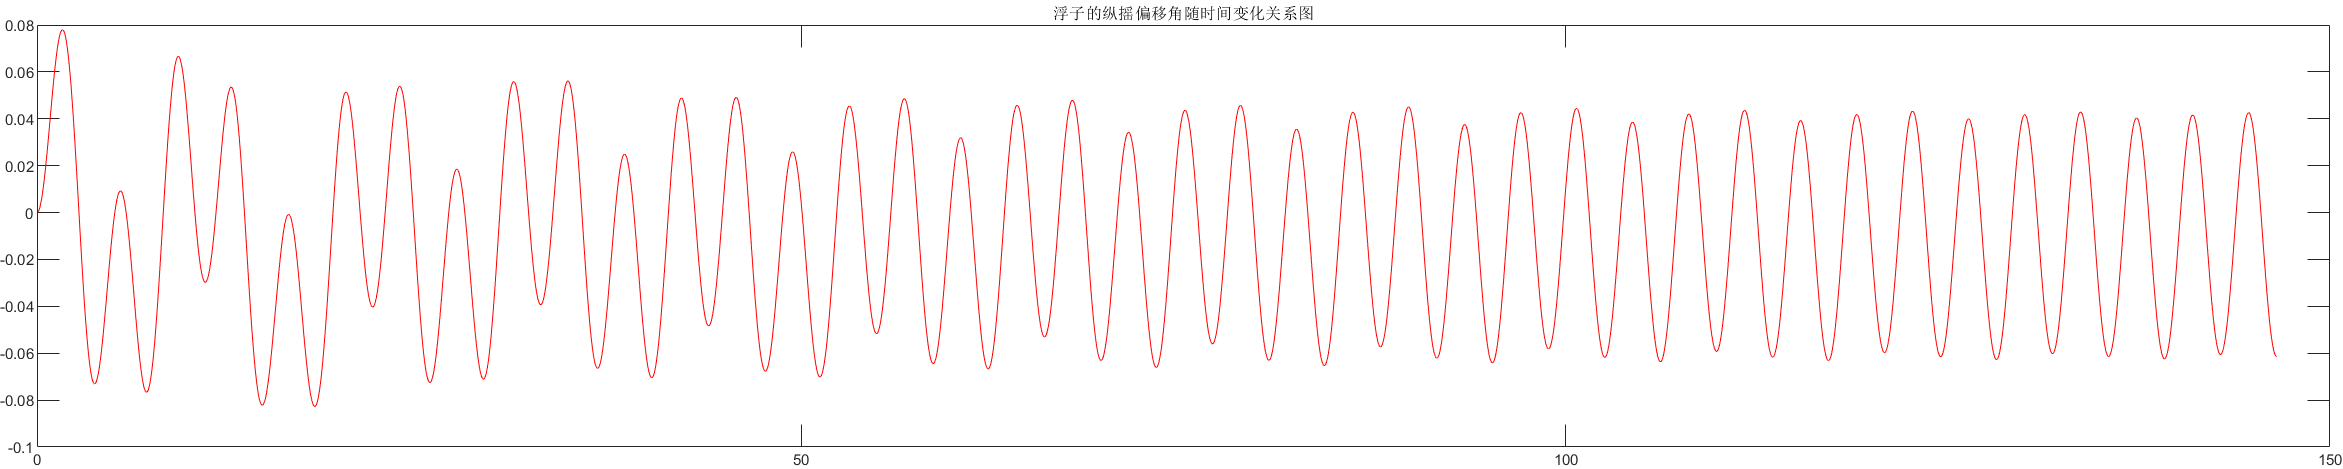
\includegraphics[scale=0.3]{问题3-2.png}
  %  \caption{2}
%\end{figure}

%\begin{lstlisting}

%\end{lstlisting}

%%%%%%%%%%%%%%%%%%%%%%%%%%%%%%
\end{document}
\end